%%%%%%%%%%%%%%%%%%%%%%%%%%%%%%%%%%%%%%%%%%%%%%%%%%%%%%%%%%%%%%%%%%%%%%%%%%%
%                                                                         %
%			TEMPLATE LATEX PER TESI                                       %
%			______________                                                %
%                                                                         %
%           Ultima revisione: 24 giugno 2019                              %
%           Revisori: G.Presti; L.A.Ludovico; F. Avanzini                 %
%                                                                         %
%%%%%%%%%%%%%%%%%%%%%%%%%%%%%%%%%%%%%%%%%%%%%%%%%%%%%%%%%%%%%%%%%%%%%%%%%%%

\documentclass[12pt,italian]{report}
\usepackage{tesi}

%
%			INFORMAZIONI SULLA TESI
%			DA COMPILARE!
%

% CORSO DI LAUREA:
\def\myCDL{Corso di Laurea triennale in\\Informatica}

% TITOLO TESI:
\def\myTitle{Riconoscimento di volti \\tramite insiemi fuzzy}

% AUTORE:
\def\myName{Tommaso Amadori}
\def\myMat{Matr. Nr. 892859}

% RELATORE E CORRELATORE:
\def\myRefereeA{Prof. Dario Malchiodi}
\def\myRefereeB{Prof. Anna Maria Zanaboni}

% ANNO ACCADEMICO
\def\myYY{2018-2019}

% Il seguente comando introduce un elenco delle figure dopo l'indice (facoltativo)
%\figurespagetrue

% Il seguente comando introduce un elenco delle tabelle dopo l'indice (facoltativo)
%\tablespagetrue

%
%			PREAMBOLO
%			Inserire qui eventuali package da includere o definizioni di comandi personalizzati
%

% Package di formato
\usepackage[a4paper]{geometry}		% Formato del foglio
\usepackage[italian]{babel}			% Supporto per l'italiano
\usepackage[utf8]{inputenc}			% Supporto per UTF-8
%\usepackage[a-1b]{pdfx}			% File conforme allo standard PDF-A (obbligatorio per la consegna)

% Package per la grafica
\usepackage{graphicx}				% Funzioni avanzate per le immagini
\usepackage{hologo}					% Bibtex logo with \hologo{BibTeX}
%\usepackage{epsfig}				% Permette immagini in EPS
%\usepackage{xcolor}				% Gestione avanzata dei colori

% Package tipografici
\usepackage{amssymb,amsmath,amsthm} % Simboli matematici
\usepackage{listings}				% Scrittura di codice

% Package ipertesto
\usepackage{url}					% Visualizza e rendere interattii gli URL
\usepackage{hyperref}				% Rende interattivi i collegamenti interni
\usepackage{algorithm}
\usepackage[noend]{algpseudocode}
\usepackage{amsmath}
\usepackage{amsfonts}
\usepackage{verbatimbox}

\setcounter{secnumdepth}{3}
\setcounter{tocdepth}{3}
\begin{document}

% Creazione automatica del frontespizio
\frontespizio
\beforepreface

% 
%			PAGINA DI DEDICA E/O CITAZIONE
%			facoltativa, questa è l'unica cosa che dovete formattare a mano, un po' come vi pare
%

         
% 
%			PREFAZIONE (facoltativa)
%

%\prefacesection{Prefazione}
%Le prefazioni non sono molto comuni, tuttavia a volte capita che qualcuno voglia dire qualcosa che esuli dal lavoro in s\'e (come un meta-commento sull'elaborato), o voglia fornire informazioni riguardanti l'eventuale progetto entro cui la tesi si colloca (in questo caso \`e probabile che sia il relatore a scrivere questa parte).

%
%			RINGRAZIAMENTI (facoltativi)
%


%
%			Creazione automatica dell'indice
%

\afterpreface

% 
%			CAPITOLO 1: Introduzione o Abstract
% 

\chapter{Apprendimento automatico}
\label{cap:apprendimento_automatico}
Il Machine Learning (ML) insegna ai computer a compiere attività in modo naturale come gli esseri umani o gli animali: imparando dall’esperienza. In sostanza, gli algoritmi di ML usano metodi matematico-computazionali per apprendere informazioni direttamente dai dati, senza modelli matematici ed equazioni predeterminate. Gli algoritmi di ML migliorano le loro prestazioni in modo ``adattivo” mano a mano che gli ``esempi" da cui apprendere aumentano. Cerchiamo allora di capire cos’è il ML, come funziona e quali sono le sue applicazioni.
\section{Approcci}
\label{sec:approcci}

I tipi di algoritmo del ML differiscono nel loro approccio, nel tipo di dati che utilizzano, che producono e nel tipo di attività o di problema che devono risolvere. Il ML può generalmente essere suddiviso in tre macro categorie: 
\begin{itemize}
	\item supervisionato,
	\item non supervisionato,
	\item apprendimento con rinforzo.
\end{itemize}
A queste si aggiunge solitamente una quarta categoria denominata semi-supervisionato.


\subsection{Supervisionato}

L'approccio supervisionato è una tecnica che prevede di lavorare su un insieme di dati associati ad etichette definite dall'utente. Le etichette sono delle classi (o gruppi) entro le quali sono suddivisi i dati. Sapendo che ogni dato è associato a un'etichetta si vuole arrivare a cogliere la relazione che vi è tra dati ed etichette, così da poter predire le etichette a partire dai dati, anche lavorando con dati non visti durante la fase di apprendimento.
%da cui possa imparare a riconoscerne le varie differenze e in seguito a fare una predizione sulla possibile classificazione. 
Questa tecnica può fornire due diversi tipi di risultati: discreti o continui. Per comprendere meglio questo concetto proviamo a fare un esempio.

Consideriamo delle diagnosi mediche fatte su una serie di pazienti. Analizzando le diagnosi un medico è in grado di definire se il paziente è in salute o meno. Da qui possiamo estrapolare quindi due etichette differenti per il nostro caso: ``in salute" e ``malato". Fornendo come input a un classificatore questo insieme di dati con le rispettive etichette appena definite, il calcolatore, tramite un'algoritmo supervisionato, sarà in grado di fornire delle predizioni sulla possibile etichetta da attribuire ad ogni nuova diagnosi.

E' importante che vi sia a disposizione una quantità consistente di dati in input. In altre parole, è importante che vi siano molti dati da analizzare, perché quando questo non succede la capacità di predizione del sistema che si ottiene è spesso di scarsa qualità.

In questo esempio abbiamo utilizzato solamente le classi ``in salute" e ``malato", ma nulla ci vieta di definirne una terza o una quarta. Ad esempio possiamo etichettare un paziente come ``asmatico" o ``diabetico".
Nel caso in cui non vogliamo avere una classificazione della salute del paziente, ma vogliamo quantificare l'aspettativa di vita, non è più possibile ricorrere a dei classificatori. Da qui nasce la necessità di passare da un valore discreto ad un valore continuo, pertanto si utilizza un modello diverso ovvero i regressori che costituiscono un modello per predire valori continui. Ad esempio, potremmo voler quantificare, data una specifica diagnosi, il tempo di guarigione per un paziente malato che per definizione si definisce su una scala di numeri continua.

I modelli di ML supervisionati hanno l'obiettivo di eseguire, con la maggior precisione possibile, una predizione su dati nuovi, mai visti prima. Per raggiungere questo scopo dobbiamo assicurarci che il modello produca stati lontani sia dal sovra-adattamento (\emph{overfitting}) che dal sotto-adattamento (\emph{underfitting}). 

L'\emph{overfitting} si verifica quando il modello tende ad adattarsi in maniera eccessiva ai dati che gli sono stati forniti per allenarsi, non permettendo la generalizzazione a nuovi insiemi di dati. 
L'\emph{underfitting} invece, si verifica nel caso contrario dell'\emph{overfitting}, quando il modello si basa su schemi troppo semplici e poco robusti, il che comporta la definizione di regole con scarsa qualità per la predizione di nuovi elementi.

\begin{table}[h!]
	\center
	\caption{Statistica per determinare l'acquisto di una nuova barca}
	\label{table_customers}
	\vspace{3 mm}
	\begin{tabular}{|c|c|c|c|c|c|}
		\hline
		Età & Macchine &  Case possedute & Figli & Stato civile & Barca    \\
		\hline
		66 & 1 & Sì & 2 & Vedova & Sì \\
		52 & 2 & Sì & 3 & Sposato & Sì \\
		22 & 0 & No & 0 & Sposato & No \\
		25 & 1 & No & 1 & Single & No \\
		44 & 0 & No & 2 & Divorziato & No \\
		39 & 1 & Sì & 2 & Sposato & No \\
		26 & 1 & No & 2 & Single & No \\
		40 & 3 & Sì & 1 & Sposato & No \\
		53 & 2 & Sì & 2 & Divorziato & Sì \\
		64 & 2 & Sì & 3 & Divorziato & No \\
		58 & 2 & Sì & 2 & Sposato & Sì \\
		33 & 1 & No & 1 & Single & No \\
		\hline
	\end{tabular}
\end{table}

Per esemplificare prendiamo spunto da un caso riportato in \cite{intro_machine_learning}. Basandoci sulla Tabella \ref{table_customers} vediamo quali sono i problemi generabili dall'\emph{overfitting} e dall'\emph{underfitting}. Supponiamo di voler predire se un cliente vorrà acquistare una barca. Osservando attentamente la tabella si può notare che applicando la regola: ``Se un cliente ha più di 45 anni, ha meno di 3 figli o non è divorziato, allora vorrà comprare una barca", tutte le predizioni (su questo dataset) saranno corrette.

Ma questo significherebbe anche che se in futuro un cliente C volesse comprare una barca e non rispettasse la regola sopra definita (magari perché ha semplicemente 44 anni o perché ha 4 figli), la predizione del sistema sarebbe ``C non vuole comprare una barca", quindi errata. Questo è il caso dell'\emph{overfitting}: stabilire le regole di predizione su troppi dati, in maniera troppo rigida.

Lo stesso si può fare al contrario, ossia quando le regole di predizione adottate dal modello si basano su pochi dati e/o le regole sono troppo vaghe. Supponiamo che il sistema identifichi un cliente come possibile acquirente di una barca se segue la seguente regola: ``Se un cliente ha una casa allora vorrà comprare una barca". È naturale, leggendo la regola, pensare che questa sia eccessivamente generica. Questo è il caso dell'\emph{underfitting}, ossia il caso in cui si definisce un modello che segue regole troppo vaghe, regole che portano a una scarsa qualità di predizione.

Quindi quello che vogliamo trovare è un modello che si posizioni a metà tra l'\emph{overfitting} e l'\emph{underiffing}. La complessità del modello, ossia quante e quali variabili vanno considerate, è un importante aspetto da considerare. Con un modello troppo ``semplice" si rischia di utilizzare dati poco significativi per effettuare predizioni. %Se ne utilizziamo troppe poche rischiamo di a sufficienza per fare predizioni corrette. 
Al contrario, quando è troppo complesso, rischiamo di utilizzare troppe variabili che non permettono di focalizzarci su quelle che sono davvero significative, il che può compromettere la performance del modello. In Figura \ref{fig:tradeoff_img} è possibile osservare quanto appena detto. L'asse orizzontale rappresenta la complessità del modello mentre quella verticale rappresenta l'accuratezza della predizione effettuata dello stesso. La curva blu raffigura l'accuratezza della predizione sui dati di allenamento e, analogamente a questa, la curva verde rappresenta l'accuratezza sui dati che non sono stati usati durante la fase di allenamento. Nel caso di una scarsa complessità del modello avremo un'accuratezza di predizione bassa in entrambi i casi. Con il crescere della complessità del modello (e quindi con il crescere della varietà di dati da poter utilizzare) notiamo che la curva blu aumenta il suo livello di precisione, mentre quella verde raggiunge il picco quando si trova ad un giusto compromesso di complessità, superato il quale torna a decrescere. Il picco di cui parliamo è lo \emph{Sweet spot}, cioè il punto che rappresenta il miglior compromesso tra precisione nella predizione e complessità del modello in caso di dati mai visti. La curva verde decresce quando la complessità diventa eccessiva. Con un numero eccessivo di variabili da considerare si rischia infatti di far perdere rilievo alle variabili più importanti tra tutte quelle considerate.%maggiore sarà la complessità e maggiori saranno le variabili da considerare, il che spesso influisce negativamente sui risultati ottenuti su dati diversi da quelli di allenamento.

\begin{figure} [h!]


	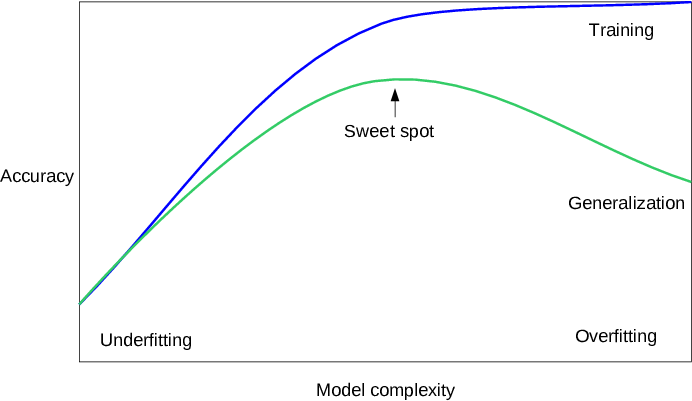
\includegraphics[scale=0.5]{../img/tradeoff_overfitting_underfitting.png}
	\caption{Trade-off tra overfitting e underfitting}
	\label{fig:tradeoff_img}
\end{figure}

% TODO: dal libro

\subsubsection{k-Nearest Neighbor}

Vediamo nello specifico uno dei più semplici algoritmi di ML: \emph{k-Nearest Neighbor} (k-NN). Questo è un algoritmo utilizzato sia per la classificazione che per la regressione. In entrambi i casi l'algoritmo si basa sul parametro $k$ fissato. Esso definisce il numero di vicini da prendere in considerazione per fare la predizione.


\begin{figure}[h!]
	\center
	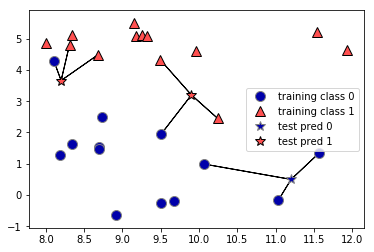
\includegraphics[scale=0.7]{../img/knn_classifier}
	\caption{Classificazione tramite k-NN di 3 elementi. Le stelle rosse rappresentano una classificazione rispetto alla classe 1 (dei triangoli) mentre le stelle blu rappresentano una classificazione rispetto alla classe 0 (dei cerchi).}
	\label{fig:knn_classifier}
\end{figure}

Supponiamo di avere due \emph{feature} (o caratteristiche), per semplicità, $ \mathrm{feature_0} $  e $ \mathrm{feature_1} $ le quale descriveranno -- insieme alla classe -- ogni record del nostro dataset.  Nel caso di classificazione tramite il k-NN in Figura \ref{fig:knn_classifier} è mostrato come un elemento non ancora etichettato venga classificato in base al tipo predominante dei suoi vicini. La scelta di $ k $ è quindi l'unica, ma fondamentale, scelta da prendere per determinare la precisione nella predizione dei futuri elementi.

\begin{figure}[h!]
	\center
	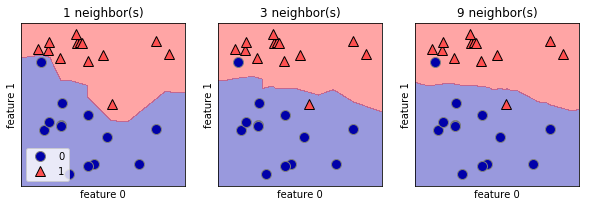
\includegraphics[scale=0.55]{../img/knn_comparison}
	\caption{Risultati di un classificatore k-NN, per diversi valori del parametro $k$ su un medesimo dataset. I cerchi e i triangoli indicano le osservazioni del dataset appartenenti a due classi, mentre le aree blu e rosse indicano gli esiti della classificazione.}
	\label{fig:knn_difference}
\end{figure}


In Figura \ref{fig:knn_difference} viene mostrato come influisce la scelta di differenti parametri $ k $ su uno stesso campione.

Questo algoritmo è spesso utilizzato con un $ k $ dispari per escludere casi di indecisione e quindi poter sempre definire la classe del nuovo dato.

Nel caso di regressione tramite il k-NN, il risultato sarà pari alla media dei valori target dei $ k $ più vicini.
\begin{figure}[h!]
	\center
	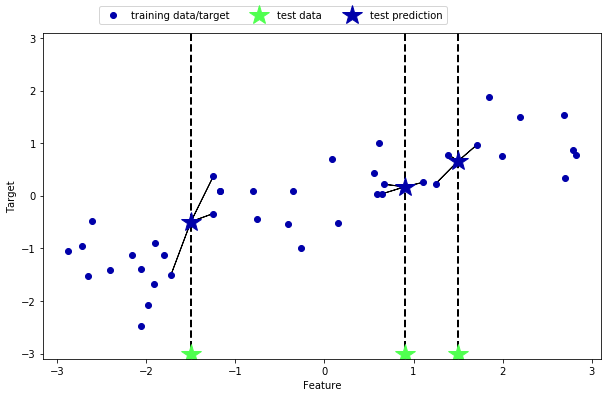
\includegraphics[scale=0.6]{../img/knn_regressor}
	\caption{Risultato di un regressore k-NN, per $k$ pari a 3. I cerchi indicano le osservazioni del dataset, le stelle verdi indicano il nuovo elemento da predire e le stelle blu gli esiti della predizione.}
	\label{fig:knn_regressor}
\end{figure}
Immaginiamo di avere, nel nostro dataset, due \emph{feature} per ogni elemento: $ \mathrm{Target} $ e $ \mathrm{Feature} $. $ \mathrm{Feature} $ rappresenta il valore su cui vogliamo basare il modello e $ \mathrm{Target} $ il valore che vogliamo predire. Prendendo ad esempio un $ k $ pari a 3 otteniamo (come vediamo in Figura \ref{fig:knn_regressor}) che il nuovo elemento da predire (la stella verde) avrà come valore $ \mathrm{Target} $ (la stella blu) la media dei $ \mathrm{Target} $ dei 3  elementi più vicini sull'asse delle ascisse (l'asse delle \emph{feature}).


\subsubsection{Modelli lineari}
I modelli lineari sono una classe di modelli che cercano di effettuare predizioni utilizzando una funzione lineare basata sull'insieme delle \emph{feature} dell'elemento da analizzare. 
Nel caso della regressione, la funzione di cui parliamo è definita come segue:
\[ y = w_{0}x_{0} + w_{1}x_{1} + ... + w_{n}x_{n} + b ,\]
dove $n$ è il numero di \emph{feature}, $x_{i}$ le \emph{feature}, $ w_{i} $ i pesi da attribuire a queste ultime e $ b $ un termine noto.
Prendendo una sola \emph{feature} (quindi $ n $ pari a 1), $ y $ risulterebbe:

\[ y = w_{0}x_{0} + b,\]
che è esattamente la funzione di una linea retta, dove $ w_{0}$ è il coefficiente angolare e $ b $ è lo scostamento dall'origine degli assi.

Riprendendo l'esempio precedente, supponiamo che si voglia quantificare il numero dei giorni necessari per guarire un paziente malato.
Supponiamo inoltre, per semplicità, di avere una sola caratteristica indicante l'età del paziente.
Nel grafico in Figura \ref{fig:linear_regression} è rappresentato il dataset dei pazienti le cui coordinate sono l'età sull'asse delle ascisse e i giorni di guarigione sull'asse delle ordinate.

È possibile tracciare una retta denominata retta di regressione che approssima tutti i punti definiti nel dataset. 

\begin{figure}[h!]
	\center
	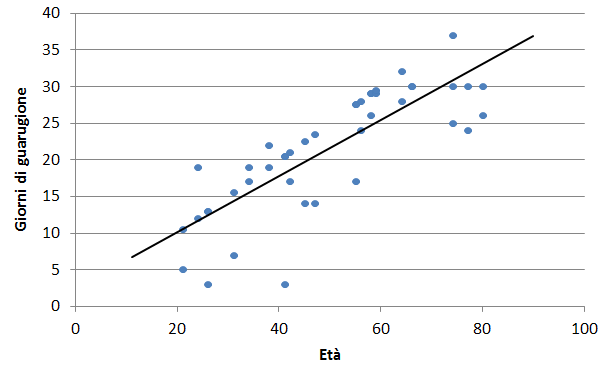
\includegraphics[scale=0.6]{../img/linear_regression}
	\caption{Linear regression}
	\label{fig:linear_regression}
\end{figure}

I modelli lineare si possono applicare anche al contesto della classificazione, modificando leggermente la loro formulazione ovvero introducendo degli intervalli per definire a quale classe appartiene il singolo caso. Nella classificazione binaria ad esempio, la formula risulterebbe come segue:
\[ y = w_{0}x_{0} + w_{1}x_{1} + ... + w_{n}x_{n} + b > 0, \]
dove, supponendo di avere le classi $ \mathrm{C_1} $ e $ \mathrm{C_0} $, se la $ y $ fosse maggiore di $ 0 $, l'oggetto descritto dagli $x_{i}$ verrebbe classificato come $ \mathrm{C_1} $, altrimenti come $ \mathrm{C_0} $.
%
%Nella figura xxx è mostrato l'esempio appena citato, dove i cerchi sono la classe 0 e i triangoli la classe 1.

\subsubsection{Support Vector Machine}
Le Support Vector Machine (SVM) sono una classe di modelli che si occupa di individuare un iperpiano utile a separare i punti in uno spazio e quindi dividerli in diversi gruppi. 

Il primo problema che le SVM devono risolvere è capire quale sia l'iperpiano che suddivide nel modo ``migliore" i dati. 
%Per capire come l'algoritmo definisca ``migliore" un certo sistema di suddivisione.

\begin{figure}[h!]
	\center
	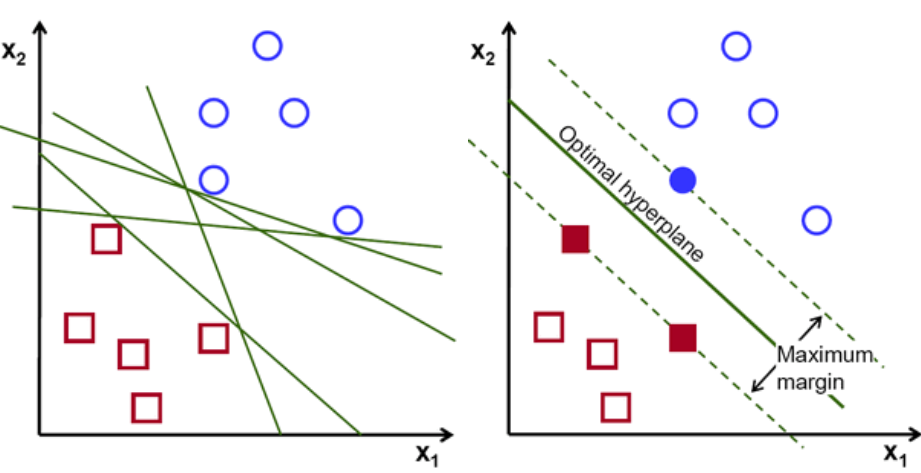
\includegraphics[scale=0.4]{../img/svc} %https://medium.com/@george.drakos62/support-vector-Machine-vs-logistic-regression-94cc2975433f
	\caption{Possibili iperpiani che dividono lo spazio (a sinistra) e iperpiano ``migliore" (a destra)}
	\label{fig:svc}
\end{figure}

Nel grafico di sinistra della Figura \ref{fig:svc} è possibile notare due gruppi distinti di punti (i cerchi blu e i quadrati rossi), che possono essere divisi dagli iperpiani raffigurati con linee verdi. Queste linee sono candidate ad essere i ``migliori" divisori per i due insiemi ma per decidere quale sia il migliore si considerano i punti P più vicini a ogni iperpiano I. Questi punti vengono definiti vettori di supporto (o \emph{support vector}). Per ogni iperpiano I e i relativi vettori di supporto V, viene calcolata la distanza tra I e V che viene chiamato ``margine". Si definisce quindi iperpiano migliore, l'iperpiano che riesce a massimizzare il margine dai rispettivi vettori di supporto. Nell'immagine destra in Figura \ref{fig:svc} mostra l'iperpiano ``migliore" ovvero l'iperpiano che massimizza il ``margine".

Nei casi reali capita spesso che lo spazio non è linearmente separabile. Per ovviare a questo problema si ricorre alle funzioni \emph{kernel} che sono in grado di mappare dei vettori da uno spazio $n$-dimensionale a uno spazio $m$-dimensionale.
Supponiamo il caso, rappresentato in Figura \ref{fig:svc_non_linear}, dove si hanno due sole dimensioni ma dove non è possibile suddividere i punti con una semplice linea.

\begin{figure}[h!]
	\center
	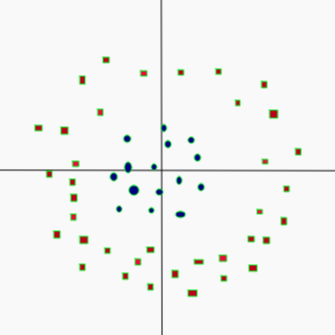
\includegraphics[scale=0.5]{../img/svc_non_linear} %https://medium.com/@george.drakos62/support-vector-Machine-vs-logistic-regression-94cc2975433f
	\caption{Dati non divisibili linearmente}
	\label{fig:svc_non_linear}
\end{figure}

Tramite una funzione \emph{kernel} trasformiamo i punti definiti dalle coordinate $x$ e $y$, in punti aventi coordinate $x$, $y$ e $z$. Questa trasformazione è conosciuta come trucco del \emph{kernel} (o \emph{kernel trick}). Essa permette di trasformare uno spazio $n$-dimensionale in uno spazio $m$-dimensionale, dove $m$ è spesso più grande di $n$. Così facendo possiamo rappresentare l'insieme in uno spazio tridimensionale e tracciare un iperpiano che suddivide in modo lineare i punti nello spazio, per poi ridefinirlo secondo le due dimensioni iniziali di partenza.
Aggiungiamo quindi una terza dimensione $z$ e definiamola come segue:
%Come esplicato in \cite{towards_data_science},
%TODO: refrenzia il post(https://towardsdatascience.com/https-medium-com-pupalerushikesh-svm-f4b42800e989), riporto l'esempio esplicativo:
%presi dei punti in uno spazio bidimensionale capita che questi non siano suddivisibili tramite una retta.

\[ z = x^2 + y^2.\]

Il risultato ottenuto è mostrato in Figura \ref{fig:svc_on_z_axis} e da esso si evince che si possono facilmente dividere i punti nelle due classi utilizzando una retta di equazione

\[ z = k ,\]
dove $k$ è una costante.

Quindi quando ci si trova davanti a problemi di suddivisione dell'iperspazio bisogna spesso ricorrere al trucco del \emph{kernel}. 

\begin{figure}[h!]
	\center
	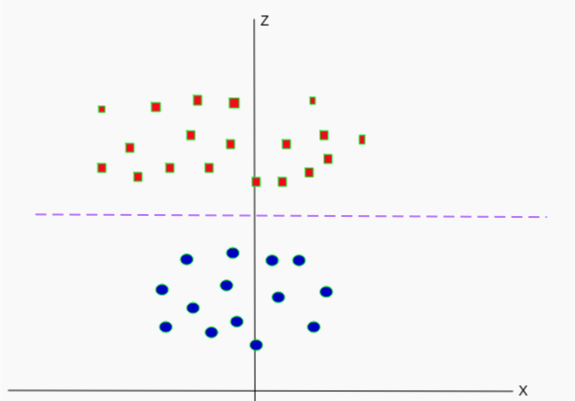
\includegraphics[scale=0.4]{../img/svc_on_z_axis} %https://medium.com/@george.drakos62/support-vector-Machine-vs-logistic-regression-94cc2975433f
	\caption{Dati visti sull'asse z}
	\label{fig:svc_on_z_axis}
\end{figure}

%SVMQuesto trucco prevede anche dei parametri $ C $ e $ \gamma $, detti iperparametri (o parametri di tuning).
%Essi influiscono sulla selezione dell'iperpiano che si va ad ottenere nello spazio inziale:
%\begin{itemize}
%	\item $C$: è il parametro che consente di definire un costo nell'errore della suddivisione dei punti, vale a dire che nel caso in cui si scelga una C grande, ogni singolo errore avrà un costo elevato, andando cosi ad adattare il modello SVM nel modo più preciso possibile al training set. Adattando il modello in maniera eccessiva al training set, però, si rischierebbe di andare in overfitting e quindi comporterebbe ad una classificazione errata nel caso di esempi estranei all'insieme dei dati di allenamento. Avendo invece, una C piccola, il costo di errore sarà basso, il quale comporterà che durante l'allenamento del modello, saranno presenti diversi errori di classificazione, però, così facendo si sta generalizzando maggiormente il modello a nuovi casi da etichettare, il che può essere positivo. Vi rimando alla figura \ref{fig:tradeoff_img} che denota un buon livello di accuratezza, il quale sta a metà tra overfitting e underfitting.
	
%	\item $\gamma$: questo parametro definisce fino a che punto arriva l'influenza di un singolo esempio di allenamento. Se ha ha un valore molto elevato, allora il limite della decisione dipenderà solo dai punti molto vicini alla linea, il che si traduce effettivamente nell'ignorare alcuni dei punti che sono molto lontani dal limite della decisione. Questo perché i punti più vicini ottengono più peso e si traduce in una curva ondulata come mostrato nel grafico precedente. D'altra parte, se il valore gamma è basso anche i punti più lontani ottengono un peso considerevole e otteniamo una curva più lineare.
%\end{itemize}

\subsubsection{Alberi di decisione}

Gli alberi di decisione (o \emph{decision trees}) sono un algoritmo di classificazione o di regressione la cui logica si basa su una struttura ad albero. I nodi dell'albero rappresentano delle domande (o \emph{test}) la cui risposta è di tipo binario (vero o falso) mentre le foglie rappresentano le classi che vogliamo predire.

%L'algoritmo predispone delle domande sulla base dei dati contenuti nell'input. 
Supponiamo, ad esempio, di voler distinguere un animale tra: falco, pinguino, delfino e orso. Nell'esempio in Figura xxx l'algoritmo parte dalla domanda D: "Ha le piume?". In questo modo abbiamo definito il primo nodo N dell'albero rappresentato da D. Sapendo che i \emph{test} previsti dall'algoritmo restituiscono un output binario, da N si diramano due sotto-alberi, rappresentati dalle categorie: $ \mathrm{C_0} $(``ha le piume"); $ \mathrm{C_1} $(``non ha le piume"). Considerando gli elementi appartenenti a $ \mathrm{C_1} $ (orso e delfino) mediante un'ulteriore domanda si possono distinguere i due animali e quindi determinarne la classe di appartenenza di ciascuno di essi. Seguendo quindi la domanda, ``Ha le pinne?" se la risposta è si, si sta parlando del delfino, ovvero l'unico animale tra i quattro che non ha le piume e ha le pinne, altrimenti è l'orso. Seguendo questa logica è possibile arrivare -- con le giuste domande -- a fare delle predizioni.

Questo è un esempio eccessivamente semplificato. Nella realtà i dati che vengono analizzati hanno spesso valori di tipo continuo, quindi il \emph{test} a cui rispondono è del tipo: ``$ x $ è maggiore di $ k $?", dove $x$  rappresenta una \emph{feature} del dataset e $k$ rappresenta una costante.

Una volta definiti i \emph{test} è possibile suddividere il piano su cui rappresentiamo i dati in diverse aree, ognuna delle quali è rappresentata da una foglia (e quindi da una classe).

\begin{figure}[h!]
	\center
	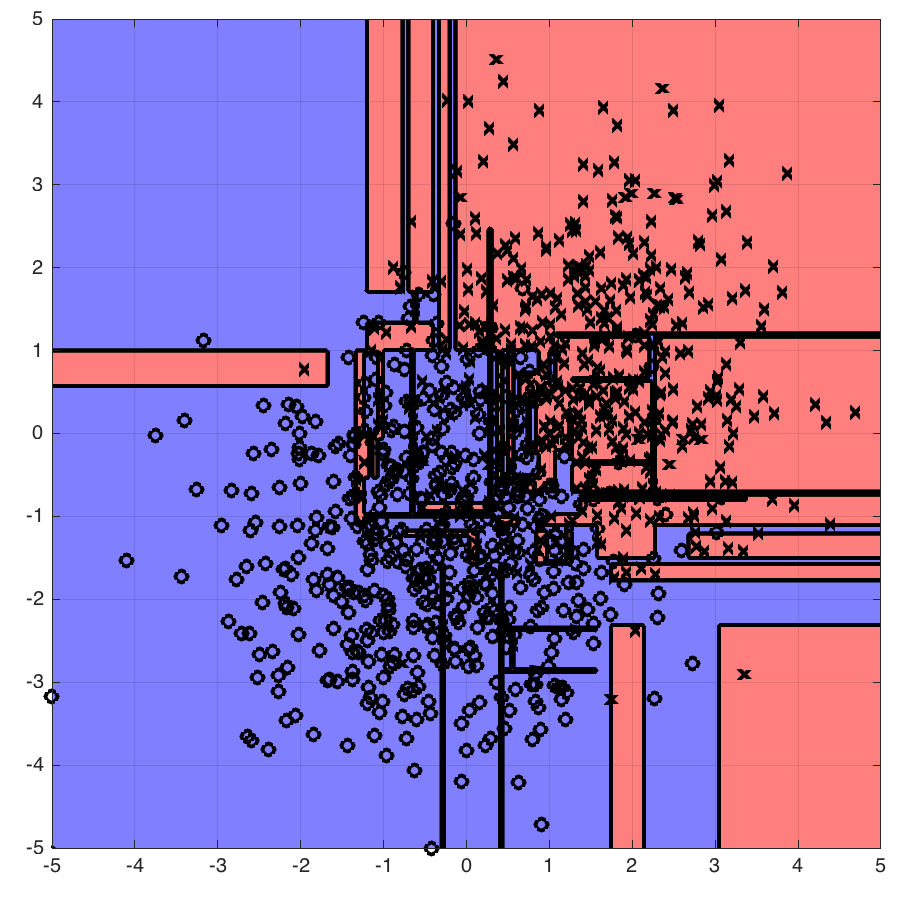
\includegraphics[scale=0.2]{../img/overfit_decision_trees1} %https://medium.com/@george.drakos62/support-vector-Machine-vs-logistic-regression-94cc2975433f
	\caption{Overfitting dei dati con l'albero di decisione}
	\label{fig:overfit_decision_trees1}
\end{figure}

Come abbiamo già visto negli altri algoritmi, il problema dell'\emph{overfitting} e \emph{underfitting} è un problema ricorrente che si presenta anche nel caso dell'albero di decisione.
Infatti se viene costruito un albero troppo dettagliato e quindi con un elevato livello di profondità il modello tende ad adattarsi in maniera eccessiva ai dati usati in fase di allenamento generando un problema di \emph{overfitting}. 

In Figura \ref{fig:overfit_decision_trees1} è raffigurato un albero di decisione sottoforma di aree su un piano bidimensionale. Nella figura è possibile osservare zone blu e rosse eccessivamente piccole le quali sono sintomo di un elevato livello di dettaglio nelle domande. Siamo quindi in presenza di un problema di \emph{overfitting}.

Analizzando un caso simile è possibile vedere tramite il grafico riportato in Figura \ref{fig:overfit_decision_trees2} come l'errore su un insieme di dati non incluso in quello di allenamento cresce con l'aumentare della profondità. Questo succede proprio perché il modello è stato allenato adattandosi in maniera eccessiva all'insieme di dati di allenamento.
\begin{figure}[h!]
	\center
	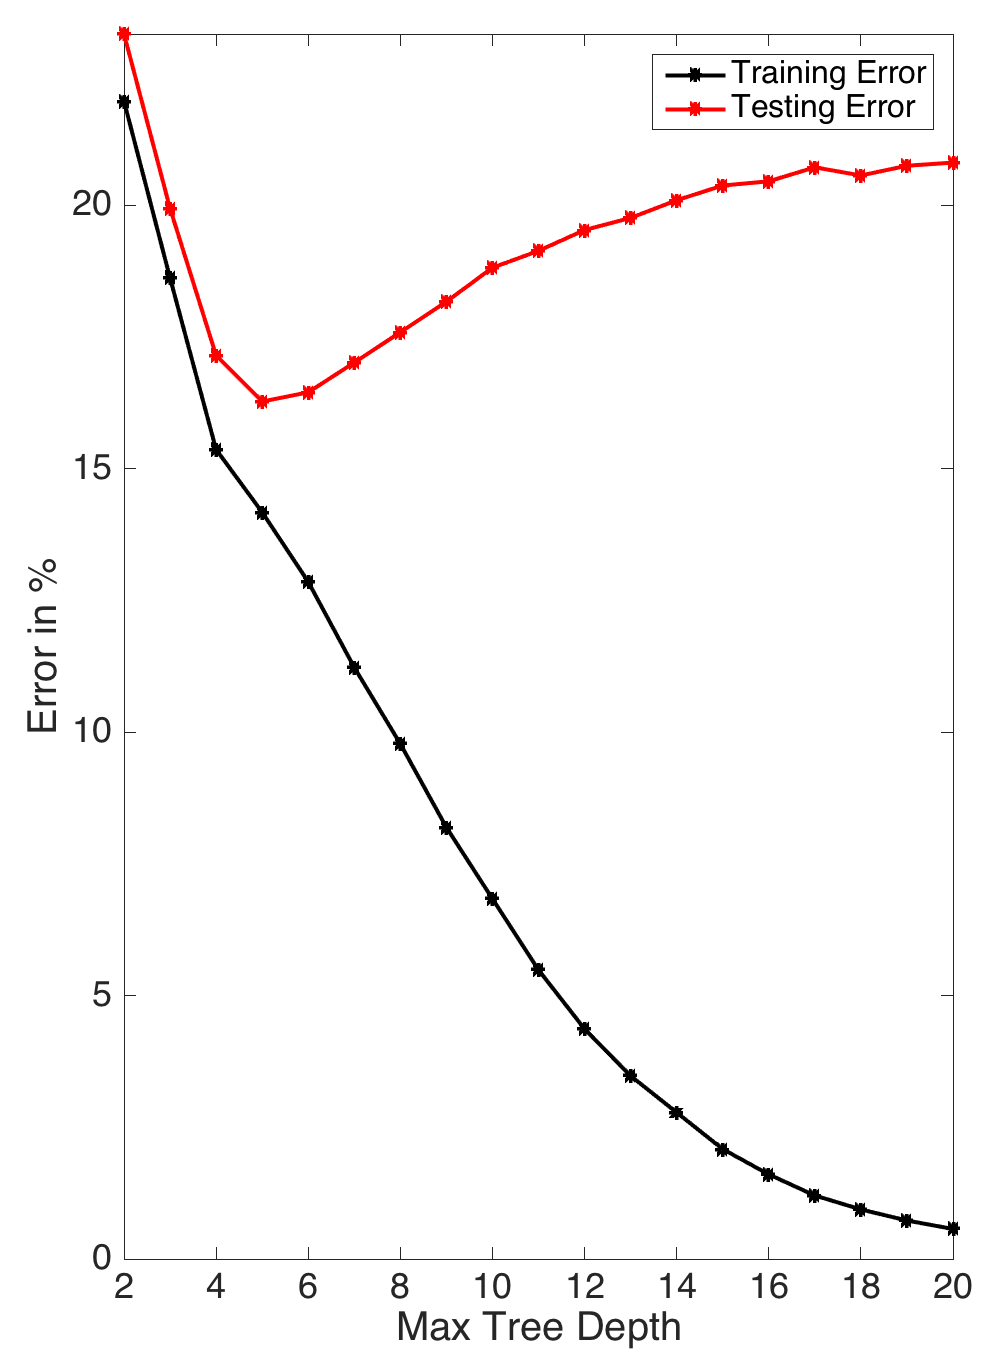
\includegraphics[scale=0.18]{../img/overfit_decision_trees2} %https://medium.com/@george.drakos62/support-vector-Machine-vs-logistic-regression-94cc2975433f
	\caption{Grafico di overfitting con l'albero di decisione. La curva nera rappresenta l'errore di precisione nella predizione di dati di allenamento mentre la curva rossa rappresenta l'errore sui dati di test}
	\label{fig:overfit_decision_trees2}
\end{figure}

Per risolvere questo problema, esistono due strategie:
\begin{itemize}
	\item far terminare lo sviluppo dell'albero dopo pochi passi (pre-potatura) ovvero limitare la profondità dell'albero mediante una variabile che tenendo conto della profondità dello stesso ne interrompa lo sviluppo al superamento di una soglia prefissata,
	
	\item rimuovere i nodi che contengono informazioni poco significative (post-potatura).
\end{itemize}

\subsection{Non supervisionato}
La tecnica non supervisionata (o \emph{Unsupervised Learning}) è il secondo importante approccio all'applicazione del ML. Cosa si intende dire con non supervisionata? Come può una macchina imparare se nessuno la guida nella scelta di decisioni?
Questa è proprio la sfida che si vuole superare con questa tecnica, ovvero far estrapolare al calcolatore, delle informazioni "nascoste" all'interno dei dati che gli vengono forniti. Queste informazioni solitamente sono dei legami, schemi o regole che i dati tendono a seguire.

Ci sono diversi utilizzi di ML non supervisionato, in questa sezione ci limiteremo a elencarne alcuni. Il principale algoritmo di \emph{Unsupervised Learning} è il clustering, ossia un algoritmo in grado di suddividere in gruppi distinti, degli elementi che hanno dati e caratteristiche in comune.

Supponiamo di aver scattato una serie di foto in cui sono raffigurate delle persone e decidiamo di caricarle su un social network. Durante il caricamento, il social su cui le stiamo caricando, visiona le foto e applica proprio un algoritmo di clustering. In che modo? L'algoritmo non sa nè chi siano le persone raffigurate nè quante esse siano. L'algoritmo andrà a cercare tutti i volti nelle foto che abbiamo caricato e, successivamente, dopo aver definito una lista di tutti i volti presenti in ogni foto, tramite un algoritmo di clustering va a cercare delle somiglianze in questi volti. Alla fine della sua esecuzione l'algoritmo avrà raggruppato le foto dove è presente lo stesso soggetto.

Un altro esempio di utilizzo ricade nella sicurezza informatica. Al giorno d'oggi i tipi di attacchi conosciuti sono probabilmente solo la punta dell'iceberg. Ricorrendo però a tecniche come questa possiamo riuscire ad individuare e bloccare attacchi tuttora sconosciuti. 
Supponiamo di essere loggati nel sito della nostra banca. Tramite il ML non supervisionato il sistema memorizzerà tutte le operazioni che faremo. Supponiamo di effettuare quotidianamente delle specifiche operazioni ad un fissato orario, in una specifica località geografica. Bene, queste informazioni vengono salvate dal calcolatore il quale le utilizzerà per creare dei cluster, ossia riconoscere quali sono le nostre operazioni comuni, riconoscendole tramite orario, località geografica e altre possibili informazioni. Supponiamo ora che un malintenzionato dall'altra parte del mondo, ad un orario differente dal nostro orario abituale, riesca ad accedere al nostro profilo bancario. L'algoritmo sarebbe in grado di notare che è in atto qualcosa di strano. Questo perché tramite il clustering nessuno gli deve dire quali sono le operazioni comuni fatte dall'utente, bensì, il computer stesso, è in grado di riconoscerle e mandare un messaggio di allarme se individua dei possibili casi anomali. 

\subsection{Semi-supervisionato}

L'approccio semi supervisionato (o \emph{semi-supervised}), non è un vero e proprio approccio, bensì una tecnica che sta a metà tra le due appena viste (supervisionato e non supervisionato). Questa tecnica consiste nel combinare le due tecniche e fornire un risultato basandosi su un input eterogeneo: classificato e non classificato.

Questo approccio risulta utile quando si ha una grande mole di dati, e gli utenti che sono in grado di classificare i dati sono utenti specializzati. Nella situazione reale, non sempre questo è possibile, proprio perché possono mancare risorse umane competenti o tempistiche adeguate per classificare tutti i dati. Esistono differenti algoritmi per l'apprendimento automatico mediante un sistema semi-supervisionato:
\begin{itemize}
	\item \emph{Self training},
	\item \emph{Multi-view training},
	\item \emph{Self-ensembling}.
\end{itemize}

Per quanto riguarda il \emph{Multi-view training}, esso mira a formare diversi modelli con diverse visualizzazioni dei dati. Idealmente, queste viste sono complementari e i modelli possono collaborare per migliorare il risultato finale. Queste viste possono differire in diversi modi, ad esempio nelle funzionalità che utilizzano, nelle architetture dei modelli o nei dati su cui i modelli vengono formati.

Il \emph{Self-ensembling}, come il \emph{Multi-view training}, punta a combinare diverse varianti dei modelli. A differenza di quest'ultimo, la diversità nei modelli non è un punto chiave perché il \emph{Self-ensembling} utilizza principalmente un singolo modello in diverse configurazioni al fine di rendere più affidabili le previsioni del modello. 

A titolo di esempio vediamo più in dettaglio l'algoritmo di \emph{Self training} che è stato uno dei primi ad essere sviluppato ed è l'esempio più diretto di come le previsioni di un modello possono essere incorporate nel training del modello.

L'algoritmo di \emph{Self training} prevede quindi di basarsi per quanto può su dei dati che sono stati preventivamente definiti secondo un particolare modo e altri che sono solamente dei dati da analizzare. Questi ultimi vengono comunque utilizzati, ma in maniera più cauta. Prima di allenare il modello, esso si concentrerà ad etichettare gli input non ancora etichettati.

Come viene spiegato nell'articolo \cite{ruder} %[https://ruder.io/semi-supervised/], 
la logica di classificazione dei dati non ancora classificati segue quanto scritto:		\\
``Formalmente, l'auto etichettamento avviene su un modello $ M $ avente un insieme $ L $ di dati di allenamento etichettato con delle etichette contenute in $ C $ e un insieme non etichettato $ U $. A ogni iterazione, per ogni $x \in U$, il modello fornisce delle predizioni su $ x $ sottoforma di probabilità $ p(x, c) $ ovvero la probabilità che $ x $ appartenga alla classe $ c $ per ogni $ c \in C $. Tra le probabilità appena calcolate, definiamo $ P(x, c) $ come la probabilità avente il valore maggiore, allora se $ P $ è più grande di una soglia $ T $, $ x $ verrà aggiunto a $ L $ con l'etichetta $ c $. Questo processo viene ripetuto per un numero fisso di iterazioni o fino a quando non ci sono più dati da etichettare.".[nota: traduzione libera del testo: nell'originale è presente una formula ceh io rendo a parole]

Di seguito vediamo uno pseduo-codice che segue quanto detto sopra:

\begin{algorithmic}[1]
	\Repeat
	\State $m \gets train\_model(L)$
	\For {$x \in U$}
	\If {$\max m(x) > \tau$}
	\State $L \gets L \cup \{(x, p(x))\}$
	\EndIf
	\EndFor
	\Until {no more predictions are confident}
\end{algorithmic}

\subsection{Apprendimento con rinforzo}
Il quarto ed ultimo approccio chiamato Apprendimento con rinforzo, o \emph{Reinforcement Learning} (RL), è un approccio che si differenzia da quelli visti fino ad ora. Questo paradigma si occupa di problemi di decisioni sequenziali, in cui l'azione da compiere dipende dallo stato attuale del sistema e ne determina quello futuro. In altre parole, questo è un sistema dinamico che può apprendere in seguito ad ogni decisione presa, a prescindere che questa sia giusta o sbagliata.

\begin{figure}[h!]
	\noindent
	\center
	\label{fig:rl_scenario}
	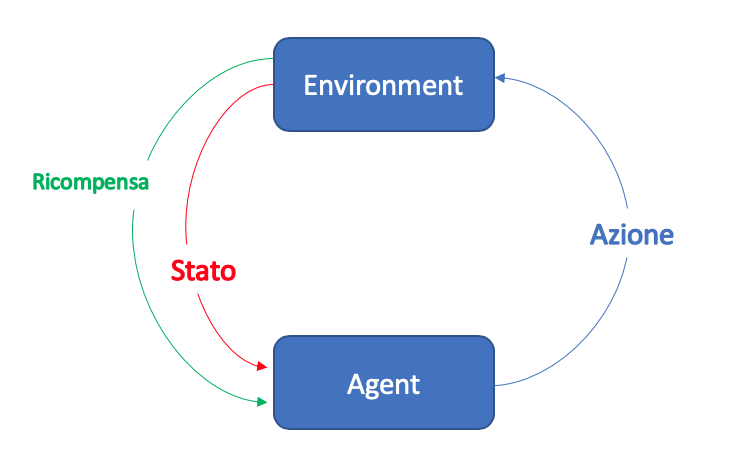
\includegraphics[scale=0.5]{../img/rl_scenario}
	\caption{Scenario RL}
\end{figure}
% (https://www.aitrends.com/education/udacitys-school-of-ai-opens-the-new-deep-reinforcement-Learning-nanodegree-program-for-enrollment/) (https://www.guru99.com/reinforcement-Learning-tutorial.html)

Quando il sistema prende una decisione, successivamente otterrà una ``ricompensa" sotto forma di punteggio, che sarà alto o basso a seconda se la decisione presa è giusta o sbagliata. Con questa logica, la macchina cercherà di fare sempre meglio per arrivare a ottenere il punteggio più alto possibile, prendendo così solo le decisioni corrette. 

\section{Ridimensionamento delle funzionalità}

Nel ML, come abbiamo visto, l'input, gioca un ruolo fondamentale nello sviluppo di un modello che riesca a predire nel modo corretto i nuovi dati che verrano esaminati da quest'ultimo.
In questo testo ci concentreremo proprio sul riconoscimento dei volti all'interno delle immagini, quindi per per parlare dell'importanza del ridimensionamento delle feature, faremo riferimento proprio all'analisi di immagini che raffigurano persone, animali o oggetti.

Spesso, ci troviamo davanti a dei dati di dimensioni eccessive, i quali comportano in primis dei problemi a livello tempistico e anche a problemi a livello computativo.

Ci basti pensare che quando si cerca di analizzare un'immagine per estrapolarne delle informazioni (riconoscimento di oggetti, persone, animali) dobbiamo prendere passare in rassegna tutti i pixel! Supponiamo di prendere anche un'immagine, a bassa risoluzione, ad esempio 500x500, significherebbe trovarsi davanti a $ 500^2 $ pixel, ovvero 250.000 elementi per una singola immagine! Questo comporterebbe quindi, di analizzare uno spazio sovra dimensionato, con, appunto 250.000 dimensioni.

Pensare ad uno spazio di quelle dimensioni è impensabile, proprio per questo ci vengono in soccorso delle tecniche che si occupano di ridurre il numero di elementi che definsicono l'oggetto, senza perdere, o meglio, estrapolando, solamente le informazioni più utili che permettono di differenziare un oggetto da un'altro.

Pensiamo ad esempio a un'immagine in cui è raffigurato il volto di una persona. E' normale pensare che non tutti i pixel siano di fondamentale importanza per riconoscere il soggetto raffigurato. Ad esempio, tutti i pixel presenti nei bordi dell'immagine saranno sicuramente da scartare in quanto non ci diranno niente sulla persona raffigurata, così come molti altri pixel che raffigurano parti poco interessanti, ad esempio lo sfondo dell'immagine. Vediamo nel dettaglio quali sono gli strumenti più utilizzati per risolvere questo tipo di problemi.


\subsection{PCA (Principal Component Analysis)}
PCA (Principal Component Analysis) è un metodo di riduzione delle dimensionalità. Lo scopo di PCA è quindi quello di diminuire il numero di variabili, limitando il più possibile la perdita di informazioni. 

In primo luogo, viene calcolata la media per ogni feature. Una volta calcolata, il vettore risultante lo faremo coincidere con l'origine degli assi, in questo modo ogni punto verrà traslato di conseguenza. A questo punto viene calcolata la retta che meglio si adatta a tutti i punti, ovvero la retta R che minimizza la somma delle distanze dei punti da R. Questa viene chiamata $ PC_{1} $. Si ripete questo passaggio per ogni dimensione, mantenendo la perpendicolarità della nuova retta (o $ PC_{n} $) rispetto all'ultima retta calcolata (o $ PC_{n-1} $). 
Una volta calcolate tutte i principal component dello spazio PCA si va a calcolare, per ognuna di esse, l'autovettore, il quale sarà utilizzato per determinare la nuova posizione di ogni punto scalandolo sul rispettivo asse. Una volta scalati tutti i punti si può calcolare la varianza per ogni asse. Il valore della varianza $\sigma$ rispetto al $ PC $ x, calcolata in percentuale, ci dice quanto pesa l'informazione contenuta su quell'asse. Questo ci permetterà quindi, di eliminare gli assi meno interessanti, ovvero gli assi con la varianza più bassa. 

Questa tecnica, oltre a semplificare il lavoro di manipolazione delle caratteristiche, aiuta a migliorare i risultati dell'algoritmo di ML. PCA aiuta gli algoritmi di ML perché estrapola le informazioni realmente utili per predire la classe o il valore da attribuire ad un oggetto. Tutte le informazioni di contorno, come ad esempio, i pixel situati sul bordo di un'immagine possono essere fuorvianti per l'algoritmo di apprendimento. Questo è il motivo per cui esso semplifica e ottimizza i valori risultanti.

PCA vede un vasto utilizzo nell'ambito di:
\begin{itemize}
	\item riconoscimento facciale
	\item image compression
	\item rilevamento di pattern in campi ad alta dimensionalità
	\item data mining
\end{itemize}

\pagebreak

\subsection{t-SNE (t-distributed stochastic neighbor embedding)}
%Documenta con delle immagini prendedole dal video https://www.youtube.com/watch?v=NEaUSP4YerM
t-SNE è una tecnica di riduzione della dimensionalità non lineare che si presta particolarmente alla mappatura di spazi ad alta dimensionalità in uno spazio a due o tre dimensioni, nel quale possono essere visualizzati tramite un grafico di dispersione. L'algoritmo modella i punti in modo che oggetti vicini nello spazio originale risultino vicini nello spazio a dimensionalità ridotta, e oggetti lontani risultino lontani.

Per spiegare il funzionamento di questo algoritmo, basiamoci su un caso semplice: un set $S$ di dati bidimensionale. Con questo esempio spiegheremo quindi il funzionamento di t-SNE e come è possibile passare da due dimensioni, ad una sola, mantenendo le corrette distanze. Per farlo ci baseremo sulle probabilità che un elemento sia vicino ad un'altro. Quindi per ogni punto x, andiamo a centrare su di esso una curva gaussiana. Per ogni altro punto $ y $  tale che:
\[ y \in S / x \]
andiamo a inserirlo sotto la distribuzione gaussiana, per poi calcolarne la probabilità di densità (o score).
%la quale verrà utilizzata per calcolare la probabilità che ogni altro elemento, sia vicino a x. 

Viene utilizzata la curva gaussiana perché lavora bene su casi come questo: restituisce un'alta probabilità se un elemento è molto vicino e una molto bassa probabilità se questo è lontano. A questo punto normalizziamo la curva per tutti i punti in modo che essi abbiano una misura proporzionata e non indipendente. La distribuzione può in realtà essere manipolata tramite una variabile chiamata perplessità, la quale va a modificare la varianza e quindi l'ampiezza della curva.
A questo punto avremo ottenuto la matrice $ M_{1} $ quadrata con tutti gli score per ogni coppia. Ora andiamo a inserire tutti i punti, in maniera casuale su un'unico asse. Analogamente a quanto appena fatto, calcoliamo la probabilità di vicinanza tra i punti, con la differenza che questa volta useremo la distribuzione di Student (in inglese t-distribution, da cui deriva la t di t-SNE). Analogamente, otterremo una seconda matrice $ M_{2} $ quadrata, la quale sarà, probabilmente, molto diversa da $ M_{1} $. L'obiettivo adesso, sarà quello di adattare la matrice $ M_{2} $ a $ M_{1} $. Così facendo riusciremo a mantenere i cluster visualizzabili nel grafico bidimensionale.

Nella seconda parte dell'algoritmo, viene usata una t-distribution perché distacca meglio i cluster nel piano generato. Se avessimo usato una distribuzione gaussiana, come nella prima parte, il risultato ottenuto sarebbe stato meno visibile, in quanto tutti i cluster si sarebbero ammassati al centro.

Questo è un esempio piuttosto semplice, ma nella realtà si possono adattare spazi a $n$ dimensioni con $ n \gg 2 $. Nel Capitolo 3 lo utilizzeremo per ridurre le dimensioni da uno spazio molto vasto, ad uno spazio bidimensionale o al più a 5 dimensioni. Vedremo quindi, utilizzando questo algoritmo, quali sono le prestazioni che riesce a fornire nel caso del riconoscimento facciale e di classificazione dei soggetti.
% 
%			CAPITOLO 2: Induzione di insiemi fuzzy
% 


\chapter{Induzione di insiemi fuzzy}
\label{ch:prova}

\section{La logica fuzzy}
La logica fuzzy (in italiano, logica sfocata), è un'estensione della logica booleana. Nella matematica booleana sono presenti solo due valori attribuili alle variabili: \emph{vero} e \emph{falso}. 
La logica fuzzy si definisce estensione della logica di Boole in quanto, al posto di prevedere solamente due possibili valori, viene previsto un insieme di valori continui compresi nell'intervallo [0, 1]. In questo intervallo lo $0$ corrisponde al valore \emph{falso} e $1$ al valore \emph{vero}. Con questa estensione oltre a poter dire \emph{vero} o \emph{falso} è possibile dire, tramite il valore di appartenenza (o grado di verità), quanto è vera una proprietà.
Quindi, data una proprietà \emph{P} e un elemento \emph{x}, si può dire:

\begin{center}
	\centering
	{

		\em{x rispetta P con valore y}
		
	}
\end{center} 
dove \emph{y} è compreso nell'intervallo $ [0,1] $.

Per fare un esempio più concreto si può pensare a tutte quelle cose che sono determinate in modo netto, in cui non esiste solo bianco o nero, bensì ci sono delle vie di mezzo più o meno vere.
Supponiamo di prendere un oggetto di cui diciamo ``essere freddo". Allora si può dire che:
\begin{itemize}
	\item un gelato ``è freddo" con valore (o grado di verità) uguale a 0.9,
	\item un bicchiere d'acqua a temperatura ambiente ``è freddo" con valore uguale a $ 0.4 $,
	\item la resistenza di una lampadina accesa ``è fredda" con valore uguale a 0.1
\end{itemize}


\section{Gli insiemi fuzzy}
La logica fuzzy è strettamente legata alla matematica degli insiemi. Gli insiemi fuzzy sono un'estensione della teoria classica degli insiemi, secondo la quale un elemento appartiene o meno ad un insieme. %Con questa estensione, analogamente al grado di verità per la logica fuzzy, si definisce con
Secondo la logica degli insiemi fuzzy $x \in [0,1]$ definisce il valore di appartenenza ad un insieme. Per $ x $ pari a $ 1 $ l'elemento è certamente incluso nell'insieme, per $ x $ pari a $ 0 $ l'elemento è sicuramente escluso dall'insieme, per tutti i valori compresi tra 0 e 1 l'appartenenza può essere più o meno forte.

Per fare un esempio definiamo lo spazio $ U $ come l'universo delle persone ed un'insieme $ A $ che include tutte le persone giovani.
Prendendo le seguenti persone di $ U $:
\begin{itemize}
	\item neonato
	\item ventenne
	\item ottantenne
\end{itemize}
si può definire per ognuna di esse un grado di appartenenza all'insieme $ A $. Ad esempio:
\begin{itemize}
	\item neonato appartiene ad $ A $ con un valore pari a 1
	\item ventenne appartiene ad $ A $ con un valore pari a 0.8
	\item ottantenne apparteiene ad $ A $ con un valore pari a 0.1
\end{itemize}
Formalizzando quanto appena detto, definiamo:
% si può definire una funzione del grado di appartenenza nu basata su un predicato p in uno spazio U tale che:
\[ \mu_{A}: U \rightarrow [0,1] \]
dove $ \mu_{A} $ rappresenta la funzione di appartenenza ad $ A $ ed $ U $ rappresenta lo spazio considerato. Un insieme fuzzy è definito dalle coppie ($x$,  $ \mu_{A}(x)$), quindi dall'elemento $ x $ e il relativo grado di appartenenza ad $ A $. Formalmente:
\[ A = \{  (x, \mu_{A}(x)) \mid x \in U\} \]

\section{Possibilearn}

Nel capitolo precedente abbiamo visto le diverse tecniche utilizzate nel ML. L'algoritmo che andremo a descrivere, denominato \emph{possibilearn}, si basa sull'induzione di insiemi fuzzy e ricade nell'approccio supervisionato, ovvero quella tecnica che necessita di dati preventivamente classificati per effettuare predizioni.

In questo caso per classificazione si intende il grado di appartenenza ad un certo insieme fuzzy. 
%TODO fai un esempio
%TODO definisci prima possibilearn
%TODO citazione del testo del professore
Dato un insieme $ X = \{ x_{1}, x_{2}, \ldots, x_{n-1}, x_{n}\} $ e il relativo insieme di gradi di appartenenza $ M = \{\mu_{1}, \mu_{2}, \ldots, \mu_{n-1}, \mu_{n}\} $, l'obiettivo di \emph{possibilearn} consiste nel determinare la forma dell'insieme fuzzy tramite l'utilizzo di $ X $ e $ M $.

\pagebreak
%TODO: sistema indentazione
Questo richiede di risolvere due problemi:
\begin{itemize}
	\item calcolare l'insieme fuzzy,
	\item definire i parametri per la funzione di appartenenza all'insieme fuzzy.
\end{itemize}

\subsection {Calcolo dell'insieme fuzzy}
Partendo dalle ipotesi che:
\begin{itemize}
	\item $ A $ è l'insieme fuzzy che contiene tutti gli elementi con grado di appartenenza pari a 1. Formalmente:
	\begin{center}
		\centering {
		$ 	A = \{x \in X \mid \mu_{A}(x) = 1\} $
		}
	\end{center}
	dove $ X $ è l'insieme delle immagini dei punti dello spazio originale appartenenti una ipersfera di centro $a$ e raggio $ R $ che sono mappate tramite una funzione $\phi$.
	
	\item Il grado di appartenenza $ \mu_{A}(x) $ dipenderà solo dalla distanza di $ \phi(x) $ da $ \alpha $.
\end{itemize}

Fatte queste ipotesi è possibile definire il seguente problema:
\emph{trovare la più piccola ipersfera avente centro $a$ e raggio $R$ che include tutte le x in X, per cui vale $ \mu_{A}(x) = 1 $}.


Tradotto in un modello matematico diventa un problema di ottimizzazione, la cui funzione obiettivo è:
\[ \min R^2 + C\sum_{i=1}^{n} (\xi_{i} + \tau_{i}) \]
%R 2 + C (ξ i + τ i )
dove $ C $ è una costante di cui parleremo successivamente, mentre $ \xi $ e $ \tau $ sono le variabili di scarto utilizzate nel problema di ottimizzazione.

$ \xi $ è la variabile di scarto legata al posizionamento dei punti all'interno dell'ipersfera mentre $ \tau $ è la variabile di scarto riferita al posizionamento dei punti all'esterno dell' ipersfera.

Alla funzione obiettivo descritta sopra aggiungiamo i seguenti vincoli:
\begin{equation}
\label{eq:1}
\begin{aligned}
\quad \mu_{i} \lVert \phi(x_{i}) - a \rVert ^2 \leq \mu_{i} R^2 + \xi_{i}\\
\end{aligned}
\end{equation}
\begin{equation}
\label{eq:2}
\begin{aligned}
\quad (1 - \mu_{i}) \lVert \phi(x_{i}) - a \rVert ^2 \geq (1 - \mu_{i})R^2 - \tau_{i} \\
\end{aligned}
\end{equation}
\begin{equation}
\label{eq:3}
\begin{aligned}
\quad \xi_{i} \geq 0, \tau_{i} \geq 0 \\
\end{aligned}
\end{equation}
dove possiamo notare che se il grado di appartenenza, vale a dire $  \mu_{i} $ è pari a 1, otteniamo che in (\ref{eq:1}) si ha:

\[\quad \lVert \phi(x_{i}) - a \rVert ^2 \leq R^2 + \xi_{i} \]
ossia che la distanza di $ x_{i} $ da $\alpha$ ( $\lVert \phi(x_{i}) - \alpha \rVert ^2$ ) è minore o uguale al raggio dell'ipersfera ( $R^2 + \xi_{i}$ ) e quindi è posizionato interamente ad essa.

Al contrario, se $ \mu_{i} $ è pari a $ 0 $ otteniamo che in (\ref{eq:2}) si ha:

\[ \quad \lVert \phi(x_{i}) - a \rVert ^2 \geq R^2 - \tau_{i} \]
ovvero che la distanza di $ x_{i} $ da $\alpha$  è maggiore al raggio dell'ipersfera (a meno della $i$-esima variabile di scarto $\tau_{i}$)

Passando per il duale e risolvendo i calcoli matematici, si può dimostrare che, preso qualunque punto $x \in X$ ed una funzione kernel $k$, vale:

\begin{equation}
\begin{split}
R^2(x) = k(x, x) - 2\sum_{i=1}^{n} (\alpha_{i}^* \mu_{i} - \beta_{i}^*(1-\mu_{i}))k(x, x_{i}) \\+ \sum_{i,j = 1}^{n}(\alpha_{i}^* \mu_{i} - \beta_{i}^*(1-\mu_{i}))(\alpha_{j}^* \mu_{j} - \beta_{j}^*(1-\mu_{j}))k(x_{i}, x_{j}),
\end{split}
\end{equation}
il che ci permette di calcolare la distanza tra il centro $a$ dell'ipersfera nell'iperspazio generato da $k$ nella soluzione ottimale e $\phi(x)$.

Analogamente al Support Vector Clustering in $possibilearn$ si individuano i \emph{support vector}, ossia i punti che delimitano la zona del cluster che in questo caso sono le immagini di $x $ che giacciono sulla superficie dell'ipersfera. Inoltre per tutti i punti $x$ aventi $ \mu(x) $ pari a 1 vale che la distanza di $x$ da $a$ (nella soluzione ottimale) è minore o uguale alla distanza di $x_{i}$ da $a$ per tutti i \emph{support vector} $x_{i}$.
Formalmente, definendo $ R^{*^2}(x) $ come la distanza di $x$ dal centro della sfera nella soluzione ottimale, possiamo riscrivere quanto appena detto :

\[ R^{*^2}(x) \leq R^{*^2}(s) \quad \forall x \mid \mu(x) = 1 \wedge \forall s \in S, \]
dove $S$ definisce l'insieme di tutti i support vector dell'ipersfera.
A questo punto bisogna definire il comportamento dell'insieme fuzzy per tutti i punti la cui distanza è maggiore del raggio dell'ipersfera. Per farlo dobbiamo prima definire dove questa distanza diventa sufficiente per dire che $x$ è certamente escluso dall'insieme fuzzy. In altre parole, bisogna trovare il confine oltre il quale il grado di appartenenza è pari a $0$. Possiamo definire questo confine come $\max_{x} R^{*^2}(x)$.
%Sapendo che $ R^{*^2} $ varia tra un minimo e un massimo (dipendenti da $x$), prendiamo il massimo, ossia: $\max_{x} R^{*^2}(x)$. 
%TODO: motiva perché predni il massimo
Esso verrà utilizzato per definire la distanza oltre la quale l'elemento sarà certamente escluso.

Tutto quello che succede tra questi due confini dipende da funzioni chiamate \emph{fuzzifier}. Le funzioni \emph{fuzzifier} possono assumere qualunque forma e descrivono come si comporta $ \mu(x) $ al crescere della distanza di $x$ dall'ipersfera nell'iperspazio generato dal kernel $k$. Queste funzioni, come la costante $C$ ed il kernel $k$ definiti precedentemente, vengono definiti iperparametri. 

%Nella prossima sezione parleremo dell'hyper-parameter tuning (in italiano, ottimizzazione dei parametri), quella parte del ML che consiste nell'ottimizzazione degli iperparametri che influiscono sul modello di apprendimento automatico e quindi sulla relativa predizione.

\subsection{Configurazione degli iperparametri}

%TODO: definire all'inziio del testo Machine learaning come ML
Iperparametro è un termine ricorrente quando si parla di ML. Si definisce iperparametro un dato fornito dall'esterno all'algoritmo di ML (ML). In altre parole, tutti i dati forniti dall'utente che influiscono sul design del modello sono considerati iperparametri. Questi si differenziano dai cosiddetti parametri perché questi ultimi sono semplici valori generati automaticamente dall'algoritmo stesso.

%Questo si definisce iperparametro e non semplicemente parametro per differenziare i dati che sono automaticamente generati all'interno dell'algoritmo di ML (ML) rispetto ai dati che gli vengono forniti dall'esterno (quindi dall'utente). Questi iperparametri costituiscono i dettagli del modello, i quali influiscono sulle performance di questo.
Abbiamo concluso il paragrafo precedente parlando di \emph{fuzzifier}. Il \emph{fuzzifier} è proprio un iperparametro. Fissato un insieme fuzzy $A$, esso definisce come si comporta la funzione di appartenenza per tutte le $x$ che hanno $ \mu_{A}(x) < 1 $. Tramite questa funzione, quindi, siamo in grado di dire come decresce il grado di appartenenza di $x$ ad $A$. Di seguito riportiamo degli esempi di \emph{fuzzifier}:

\begin{itemize}
	\item Linear fuzzifier ($\hat\mu_{\text{lin}}$)
	\item Crisp fuzzifier ($\hat\mu_{\text{crisp}}$)
	\item Quantile constant piecewise fuzzifier ($\hat\mu_{\text{qconst}}$)
	\item Quantile linear piecewise fuzzifier ($\hat \mu_{\text{qlin}}$)
\end{itemize}

\begin{figure}[h!]
	\center
	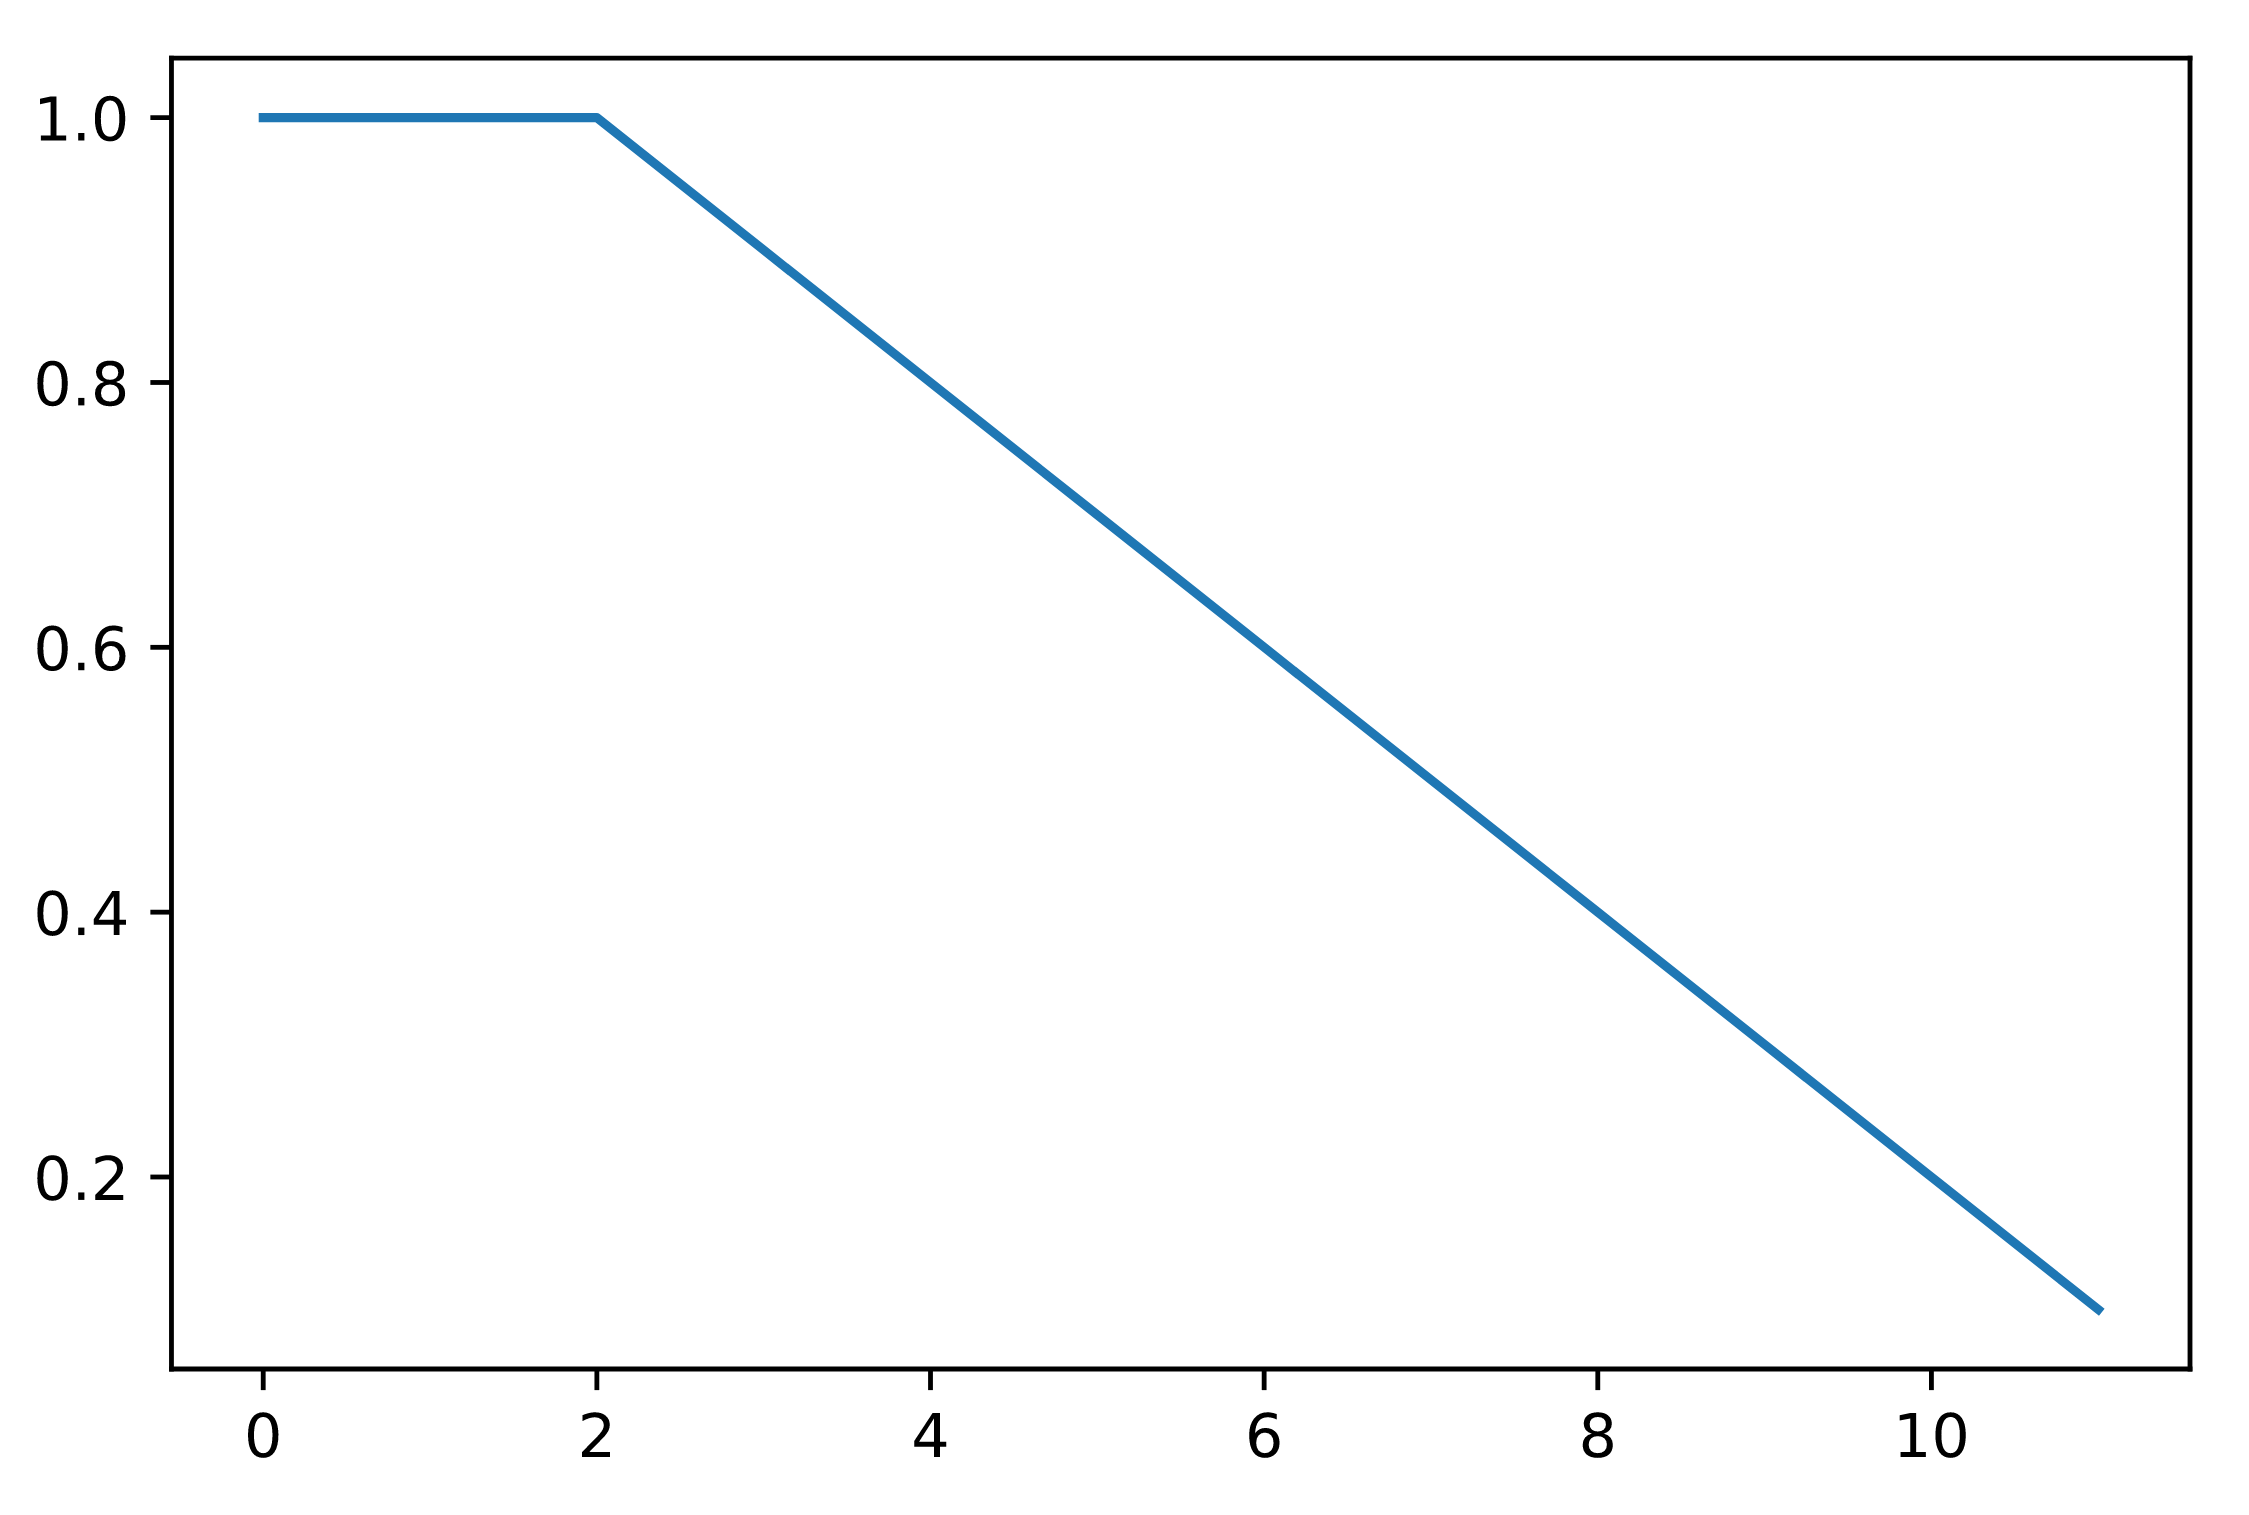
\includegraphics[scale=0.1]{../img/lin}
	\caption{Esempio di Linear fuzzifier ($\hat\mu_{\text{lin}}$)}
	\label{fig:fuzzifier}
\end{figure}

%TODO commenta gli esempi di fuzzifier
Un secondo iperparametro che troviamo in \emph{possibilearn} è la costante $C$ che compare nella funzione obiettivo:

\[ \min R^2 + C\sum_{i=1}^{n} (\xi_{i} + \tau_{i}) \]

Questa costante rappresenta un iperparametro che definisce il costo dell'errore nella classificazione degli elementi durante la costruzione dell'ipersfera. Quesa $ C$ funziona in maniera analoga alla $C$ nelle SVM (Support Vector Machine). Tanto più è grande $C$, tanto più sarà elevato il costo dell'errore nella classificazione della variabile $i$-esima. Al contrario, tanto più è piccola $C$, tanto più piccolo sarà il costo dell'errore. 

In Figura xxx%TODO: aggiiungi figura
, possiamo osservare il ruolo di questo iperparametro al variare del suo valore. In ciascun grafico della Figura al variare di $C$ osserviamo come si modifica una stessa funzione di appartenenza $\hat \mu$. 
Sapendo che la funzione obiettivo che vogliamo risolvere è una funzione di minimo, bisogna mantenere il costo più basso possibile. Questo si traduce visivamente in una funzione ``rigida" avente un cambiamento molto brusco. È facile notare che maggiore è $C$ e maggiore sarà la somiglianza di $\hat \mu$ ad una ``funzione di appartenenza" in un insieme standard.
%Non mi convince funzione di appartenenza di un insieme

[FIGURA DI FUZZIFIER DI MALCHIODI]
[FIGURA DI FUNZIONE DI APPARTENENZA DI UN INSIEME]


Esiste un ulteriore parametro che modifica la forma del \emph{fuzzifier}, questo è il kernel. Il kernel, come abbiamo visto nelle SVM è una funzione che viene utilizzata per mappare uno spazio N-dimensionale, in uno spazio M-dimensionale (dove M è spesso molto più grande di N). Esso compare nella ridefinizione della distanza di $ R^2(x) $. Questo iperparametro permette di modificare la forma di $\hat \mu$. Prendendo l'esempio in Figura xxx e una funzione kernel gaussiana, vediamo come modificando $\sigma$ (parametro della funzione kernel gaussiana) viene modificata la forma della funzione di appartenenza.

[FIGURA DI FUZZIFIER CON SIGMA MODIFICATO]

Ricapitolando in \emph{possibilearn} osserviamo tre diversi iperparametri:
\begin{itemize}
	\item $C$: per determinare il costo degli errori di classificazione in fase di definizione del fuzzy set,
	\item \emph{fuzzifier}: funzione che determina il grado di appartenenza all'insieme fuzzy,
	\item kernel: funzione utile a mappare gli elementi dallo spazio originale ad uno spazio sovra-dimensionato.
\end{itemize}

\begin{thebibliography}{9}
	\bibitem{intro_machine_learning} 
	Andreas C. Müller, Muller Andreas C, Sarah Guido. 
	\textit{Introduction to Machine Learning with Python: A Guide for Data Scientists}. 
	``O'Reilly Media, Inc.", 26 Settembre 2016
	
 	\bibitem{towards_data_science}
 	Rushikesh Pupale. \textit{Support Vector Machines(SVM) — An Overview}, \\\texttt{https://towardsdatascience.com/https-medium-com-pupalerushikesh-svm-f4b42800e989}
 	
 	\bibitem{ruder}
 	Sebastian Ruder. \textit{An overview of proxy-label approaches for semi-supervised learning}
 	\\\texttt{https://ruder.io/semi-supervised/}
	\bibitem{knuthwebsite} 
	Knuth: Computers and Typesetting,
	\\\texttt{http://www-cs-faculty.stanford.edu/\~{}uno/abcde.html}
\end{thebibliography}

\end{document}


 
